\section{Постановка проблеми}
 
Виробники автомобілів, електроніки та телекомунікаційні компанії налаштовані на створення комп’ютерних інформаційних систем на всіх транспортних засобах. Більшість автомобілів сьогодні оснащені інтерактивними інформаційними системами, включаючи високоякісні аудіо / відео системи, супутникові навігаційні системи, гарнітури телефонії та контроль над кліматом та технічним станом автомобіля \cite{art1,Kravchenko_2009,Heisterkamp_2001}.

Незважаючи на те, що більшість систем в автомобілі є дисплеєм, голосова взаємодія стає все більш широко використовуватися в автомобільних системах. Використання голосової технології в автомобілі допомагає збільшити кількість контрольованих функцій і систем, кнопки яких не можуть бути встановлені на рульовому колесі та приладовій панелі, оскільки обмежено простір. Голосова технологія також дозволяє водіям триматися руками за кермо, а очі не відривати від дороги під час взаємодії з системою \cite{art1,Kravchenko_2009,Heisterkamp_2001}.

У зв’язку з дедалі активнішим використанням природного інтерфейсу і зокрема голосу для спілкування водія з технікою зросло і значення систем голосового управління в самому автомобілі як носія інформації у системах диспетчерського контролю за рухом автотранспорту при здійсненні етапів дистрибуції «склад – дорога – точка доставки» \cite{art1}.

Саме голосова інформація в системах диспетчерського контролю за рухом автотранспорту при взаємодії із водієм потребує формалізації у випадку проведення автоматизації таких систем.

\section{Аналіз останніх досліджень і публікацій}

Для сучасних систем голосового управління існують проблеми, пов’язані з наявністю багатьох різних розмовних мов, притаманних їм діалектів та окремих формулювань, а також з індивідуальними особливостями вимови людини і її швидкістю мови. Для цього в системах голосового управління використовують різні фільтри шумів, які прибирають зайві звуки з підвищенням якості в процесі розпізнавання команд тощо \cite{Kravchenko_2009,Heisterkamp_2001,Jonsson_2009}.

Слід зазначити, що для випадку наявності достатньо потужної системи, голосову взаємодію з водієм можна використовувати для підтримання діалогу під час руху вночі, аби не дати водію заснути \cite{Kravchenko_2012}.

Підхід, який існує для голосового управління, заснований на теорії несилової взаємодії \cite{Teslia_2010} – рефлекторна система голосового управління \cite{Egorchenkov_2016,Pylypenko_2009}. Ідея, покладена в основу цього підходу, полягає в тому, щоб замість переведення голосової інформації в текстову репрезентацію, аналізувати безпосередньо інформаційну складову сказаного, визначаючи, яку з відомих реакцій потрібно виконати.

Використання таких часткових функцій голосового управління, які підвищують комфорт водія, також повинно мати певний позитивний ефект. Проте ці функції не забезпечують оптимізації саме процесів дистрибуції.

Для формалізації голосової інформації можна використати систему з двох основних модулів: автоматичного фонетичного стенографа і ядра рефлекторної системи голосового управління (РСГУ), поточна реалізація яких визначає умови їх використання в моделі голосової взаємодії водія при диспетчерському контролі за рухом автотранспорту (рис. \ref{img:rsgu_struct}) \cite{Teslia_2014,Teslia_2013}.

Застосування алгоритму фонетичного стенографа дозволяє будувати послідовність контекстів для мовного сигналу без використання будь-якого словника. Для цієї мети будується деяка генеративна граматика, яка може синтезувати всі можливі модельні сигнали безперервної мови для будь-якої послідовності фонем. В рамках побудованої моделі будується алгоритм пофонемного розпізнавання для невідомого сигналу з використанням контекстів та можливих реакцій на них.

\section{Постановка завдання}

У даній статті необхідно запропонувати метод формалізації голосової інформації в системах диспетчерського контролю за рухом автотранспорту.

\section{Виклад основного матеріалу}

У розглядаємій системі формалізації голосової інформації (рис. \ref{img:rsgu_struct}) вхідною інформацією виступає голосова команда, яка може бути представлена звуковою хвилю; вихідною ж інформацією буде виступати процес керуючого впливу на об’єкт управління, тобто відбуватиметься виконання розпізнаної команди відповідно до попередньо заданих голосом параметрам.

\begin{figure}
	\centering
	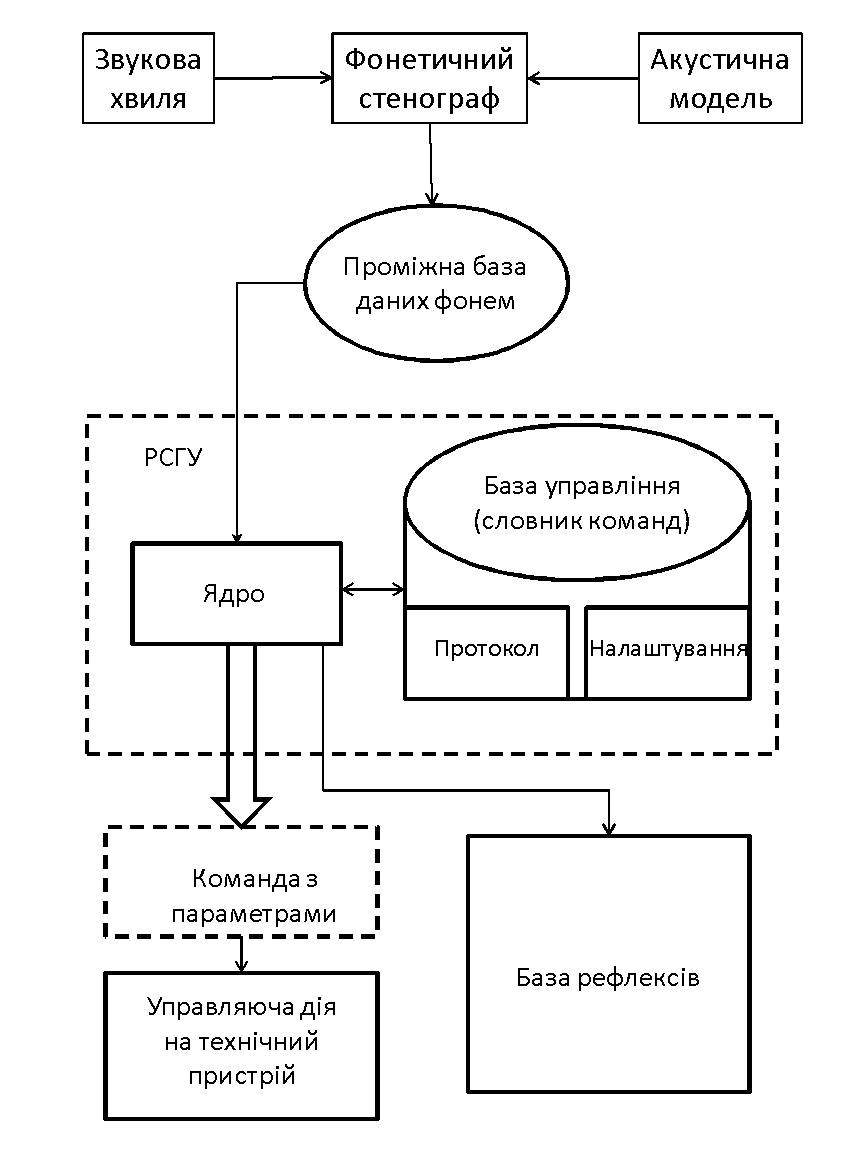
\includegraphics [width=.5\linewidth] {rsgu_struct}
	\caption{Структура системи формалізації голосової інформації в моделі голосової взаємодії водія при диспетчерському контролі за рухом автотранспорту}
	\label{img:rsgu_struct}
\end{figure}

Виконання фонетичного стенографу \cite{Teslia_2014,Teslia_2013} здійснено у вигляді бінарного додатку, набору бібліотек і конфігураційних файлів для платформи Windows, а саме ядро РСГУ виконує реалізацію інтроформаційного методу вироблення рефлексів, яке розроблено і виконане в середовищі MS Access на всіх операційних системах сімейства Windows.

Сама система формалізації голосової інформації в процесі роботи буде генерувати потрібні візуальні і голосові інформаційні повідомлення водію, це, в свою чергу, надає можливість відслідковувати процес розпізнавання команд, реакції на них і, крім того, дозволяє в реальному масштабі часу змінювати поведінку системи в разі потреби.

Докладніше ядро РГСУ описано в статті \cite{Teslia_2013}. Як альтернативу можна спробувати замінити ядро РГСУ на  згорткову нейронну мережу (ЗНМ), зберігаючи загальну структуру системи. Тобто для формалізації голосової інформації в моделі голосової взаємодії водія при диспетчерському контролі за рухом автотранспорту запропоновано використовувати згорткові нейронні мережі. У даному випадку система формалізації голосової інформації аналогічно до попередньо наведеної, складається з двох частин: фонемний стенограф та сама згорткова нейронна мережа (ЗНМ), яка працює з фонемами.

ЗНМ для роботи з фонемами найбільше нагадує ЗНМ в задачі класифікації текстів \cite{Kim_2014}, але оперує з «текстом» не по словах, а пофонемно, що схоже на роботу з текстом посимвольно \cite{Zhang_2015}.

ЗНМ дуже схожі на звичайні нейронні мережі: вони також побудовані на основі нейронів, які володіють постійно змінюваною вагою і зсувами. Кожен нейрон отримує деякі вхідні дані, виконує скалярне перетворення інформації і, в окремих ситуаціях, супроводжується нелінійністю. Як і у випадку зі звичайними нейронними мережами, вся ЗНМ висловлює одну диференційовану функцію внеску (ефективний внесок): з одного боку це необроблені фонеми, з іншого – висновок класу або групи ймовірних класів, які характеризують фонему. Також присутня функція втрати на останньому (повністю підключеному) шарі ЗНМ.

Архітектура ЗНМ робить явне припущення виду «вхідні дані є фонеми», що дозволяє закодувати певні властивості під архітектуру. Як відомо, нейронні мережі отримують вхідні дані (один вектор), після чого трансформують інформацію, проводячи її через ряд прихованих шарів \cite{Kim_2014,Zhang_2015}. Кожен прихований шар складається з безлічі нейронів, де всякий нейрон має стійкий зв’язок з усіма нейронами в попередньому шарі і де нейрони в функції одного шару повністю незалежні один від одного і не мають спільних з’єднань. Останній повнозв’язний шар називається вихідним шаром, і в настройках класифікації він демонструє число класів.

ЗНМ користуються тим, що вхідні дані складаються з фонем, і вони обмежують побудову мережі більш розумним шляхом. На відміну від звичайної нейронної мережі, шари ЗНМ складаються з нейронів, розташованих в декількох вимірах.

У роботі, за основу реалізації було взято реалізацію з відкритим вихідним кодом \cite{Britz_2015} на мові Python з використанням TensorFlow.

Структура нейронної мережі може бути представлена наступним чином.

Фонеми представлені у вигляді one-hot вектору. Фрази нормалізовані за максимальною довжиною, з використанням вектора з всіма нулями в якості заповнювача.

На відміну від роботи по словам, вкладений шар (embeding layer) відсутній, оскільки потужність множини фонем набагато нижчий ніж потужність множини слів, і такий шар не є необхідним. З іншого боку, деякі фонеми схожі на інші, а деякі ні, тому використання вкладень може бути доцільним для передачі цієї схожості, а не тільки для зниження розмірності. Навчання вкладеного шару потребує великого об’єму вхідних даних, тому в даній роботі не буде розглянуто.

Використовується комбінований згортковий шар (convolution layer), який складається з декількох паралельних одновимірних шарів з різними варіантами кроку фільтра.

Для агрегації кожного зі згорткових шарів використовується агрегаційний шар (pooling layer) з вибором одного максимального значення (1-max-pooling).

Виходи агрегаційних підшарів різного розміру кроку згортки комбінується в один вектор значень.

У якості повнозв’язного шару використовується класичний перцептрон, який може мати активаційну функцію у вигляді неспадаючих диференційованих функцій, що діють на множині дійсних чисел. У нашому випадку для функції активації використаємо ReLU:

\[
h(a) = \max(0, a),
\]

\noindent
де $a=WX+b$.

Застосування у якості функції активації ReLU дозволяє забезпечити головні переваги, які надають можливість здійснити пришвидшення навчання нейронної мережі через розрідженість та меншу величину ймовірності розмиття градієнту в порівнянні з іншими активаційними функціями. Виникнення розрідженості відбувається при значеннях a < 0. Для більшої кількості нейронів з ReLU-активацією в шарі характерна більша розрідженість отриманого результату.

Для зниження ефекту перенавчання використовується Dropout шар.

Традиційно для задач класифікації в якості функції втрат використовується кросс-ентропія. Інакше кажучи, робимо мінімізацію різниці між виходом нейронної мережі і відповідною фонемою (контекстом). Різницею, якраз і буде величина кросс-ентропії, яка визначається за наступною формулою:

\[
D(\hat{y},y)=-\sum_j y_i \ln \hat{y}_i
\]

Для навчання використовується Adam-алгоритм зворотного розповсюдження помилки із стохастичним градієнтним спуском, який дозволяє регулювати величину швидкості навчання в залежності від параметрів з виконанням більших оновлень для 32-х або 16-ти рідких параметрів і маленьких оновлень для більш частих параметрів. У даному методі використовуються накопичені значення градієнтів, що отримані на попередніх кроках, і накопичені значення квадратів градієнтів. Сам процес накопичення протікає на основі експоненціального розпаду середніх значень (EDAverage). Самі значення, що отримані на останньому кроці мають найбільший внесок для сумарного вихідного значення в порівнянні із значеннями градієнтів, що отримані на перших кроках:

\[
\bar{m_t}=\beta_1m_{t-1}+(1-\beta_1)g_t;
\]

\[
\bar{v_t}=\beta_2v_{t-1}+(1-\beta_2)g^2_t,
\]

\noindent
де $\bar{m_t}$ – середня оцінка першого моменту; $\bar{v_t}$ – середня оцінка другого моменту.

Оскільки у вищеприведених формулах констатація величин mt і vt може бути ініціалізована нулями, то виходить, що вони мають тяжіння до нулів. Таке тяжіння сильно проявляється на початкових кроках і, коли величина коефіцієнтів розпаду приймає мале значення (1 і 2~1). Для вирішення цієї проблеми на значення моментів накладається штраф:

\[
\hat{m}_t=\frac{m_t}{1-\beta_1^t};
\]

\[
\hat{v}_t=\frac{v_t}{1-\beta_2^t}.
\]

Величини отриманих значень використовуються в процесі оновлення нових параметрів на основі формули:

\[
\Theta_{t+1}=\Theta_t-\frac{\eta}{\sqrt{\hat{v}_t}+\varepsilon}\hat{m}_t.
\]

\section{Висновки}

У роботі запропоновано метод формалізації голосової інформації в системах диспетчерського контролю за рухом автотранспорту. Для формалізації голосової інформації запропоновано використання системи, що складається з двох основних модулів: автоматичного фонетичного стенографа і ядра рефлекторної системи голосового управління, поточна реалізація яких визначає умови їх використання в моделі голосової взаємодії. При використанні такої системи непотрібно створювати ніяких словників, виконувати морфологічний, синтаксичний, семантичний аналіз тексту, а також виділяти слова і команди; виникнення реакції відбувається на звуковий потік, з якого система формалізації голосової інформації в моделі голосової взаємодії водія при диспетчерському контролі за рухом автотранспорту, як і людина сама «вміє виділяти» інформативну частину за максимальною визначеністю. Також для формалізації голосової інформації запропоновано використовувати згорткові нейронні мережі. У даному випадку система формалізації голосової інформації в моделі голосової взаємодії водія при диспетчерському контролі за рухом автотранспорту містить фонемний стенограф та згорткову нейронну мережу, яка працює з фонемами. Реалізація ЗНМ виконана на мові Python з використанням TensorFlow. Нейронна мережа містить паралельні одновимірні шари з різними варіантами кроку фільтра з активаційною неспадаючою диференційованою функцією ReLU; фонеми представляються у вигляді one-hot вектору, фрази нормалізовані за максимальною довжиною, з використанням вектора з всіма нулями в якості заповнювача. Для навчання використано Adam-алгоритм зворотного розповсюдження помилки із стохастичним градієнтним спуском, який дозволяє регулювати величину швидкості навчання в залежності від параметрів. Для зниження ефекту перенавчання ЗНМ використано Dropout шар. Також побудовано алгоритм зворотного поширення помилки ЗНМ. 